\documentclass[a4paper, 11pt,reqno]{article}
\input{/Users/olivierglorieux/Desktop/BCPST/2020:2021/preambule.tex}
\usepackage{enumitem}
\geometry{hmargin=2.0cm, vmargin=2.5cm}
\lstset{basicstyle=\ttfamily, keywordstyle=\rmfamily\bfseries}
\newif\ifshow
\showtrue
\input{/Users/olivierglorieux/Desktop/BCPST/2021:2022/ifshow.tex}

\author{Olivier Glorieux}


\begin{document}

\title{Correction DS 1\\}



\vspace{1.5cm}
\begin{exercice}
Résoudre les équations et inéquations suivantes :
\begin{enumerate}
\item $\ln (2 x+3)=2 \ln (x)+\ln (3)$
\item  $\left|x^2+6 x+5\right| \leq x+5$
\end{enumerate}
\end{exercice}


\begin{correction}
\begin{enumerate}
\item On note $E$ l'équation : $\ln (2 x+3)=2 \ln (x)+\ln (3) $

L'ensemble de définition de $(E)$ est $D= ]0,+\infty[$ et  on a 
\begin{align*}
(E) \equivaut & \ln(2x+3)=\ln(3x^2)\\
	\equivaut & 2x+3 = 3x^2\\
		\equivaut & 3x^2-2x-3=0
\end{align*}
Le discriminant de $3x^2-2x+3$ est $\Delta = 40$, il y a donc deux racines réelles 
$$r_1 =\frac{2 -\sqrt{40} }{6} \quadet r_1 =\frac{2 +\sqrt{40} }{6}$$
Remarquons que $r_1$ est négatif car $2 =\sqrt{4}<\sqrt{40}$. 

Ainsi  $(E)$ admet une unique solution 
\conclusion{$\cS =\{ \frac{1+ \sqrt{10}}{3}\}$}


\item On note $E_2$ l'équation $\left|x^2+6 x+5\right| \leq x+5 $
Le discriminant du polynome $x^2+6 x+5$ est $\Delta = 16$, il y  a donc deux racines réelles :
$r_1 = -5 \quadet r_2 = -1$
et donc $$x^2 +6x+5 = (x+5)(x+1)$$

On distingue donc deux cas : 
\begin{itemize}
\item[$\bullet$]Si $x^2 +6x+5> 0$ c'est à dire : $x\in ]-\infty, -5[\cup ]-1, +\infty[$\\

On a alors $$\begin{array}{rrl}
(E_2) \equivaut& (x+5)(x+1)& \leq x+5\\
 \equivaut& (x+5)(x+1) - (x+5)&\leq 0\\
 \equivaut &(x+5)(x+1-1)&\leq 0\\
 \equivaut& (x+5)x&\leq 0
\end{array}$$



Les solutions de cette dernière inéquation  sur $\R$ sont $ [-5,0]$. Or $x\in ]-\infty, -5[\cup ]-1, +\infty[$, donc les solutions sont 
$$\cS_1= [0,-1[$$

\item[$\bullet$]Si $x^2 +6x+5\leq  0$ c'est à dire : $x\in [-5,-1]$\\

On a alors \begin{align*}
(E_2) \equivaut &-(x+5)(x+1) \leq x+5\\
 \equivaut& (x+5)(x+1) + (x+5)\geq 0\\
 \equivaut &(x+5)(x+1+1)\geq 0\\
 \equivaut& (x+5)(x+2)\geq 0\\
\end{align*}

Les solutions de cette dernière inéquation  sur $\R$ sont $  ]-\infty, -5]\cup [-2, +\infty[$. Or  $x\in [-5,-1]$, donc les solutions sont 
$$\cS_2=\{-5\} \cup [-2,-1]$$
\end{itemize}

 Finalement les solutions de $(E_2)$ sont 
 \conclusion{ $\cS =\cS_1 \cup \cS_2  =[0,-1[\cup\{-5\} \cup [-2,-1] = \{-5\} \cup [-2,0]$} 




\end{enumerate}
\end{correction}


\begin{exercice}
Calculer en fonction de $n\in \N$ : 
$$S_1 =\sum_{k=1}^{n-1} (k^2+2^k)$$
\end{exercice}

\begin{correction}
\begin{align*}
S_1&= \sum_{k=1}^{n-1} (k^2+2^k)\\
	&=\sum_{k=1}^{n-1} k^2+ \sum_{k=1}^{n-1} 2^k\\
		&=\frac{(n-1)n (2(n-1)+1)}{6}+ \sum_{k=0}^{n-1} 2^k- 2^0\\
		&=\frac{(n-1)n (2n-2+1)}{6}+ \frac{1-2^n}{1-2}-1\\	
		&=\frac{(n-1)n (2n-1)}{6} -2-2^n
\end{align*}

\conclusion{ $S_1=\frac{(n-1)n (2n-1)}{6} -2-2^n$}

\end{correction}

\begin{exercice}
\begin{enumerate}
\item Resoudre l'inéquation suivante : 
$$\sqrt{2x^2-2} \leq x \quad (E_1)$$

\item A l'aide d'un changement de variable, en déduire les solutions de  l'inéquation suivante :
$$\sqrt{2e^{2x}-2} \leq e^x \quad (E_2)$$

\end{enumerate}


\end{exercice}
\begin{correction}
\begin{enumerate}



\item L'ensemble de définition de $(E_1) $ est $D=]-\infty,-1]\cup [1,+\infty[$. 
On distingue deux cas :
\begin{itemize}
\item[$\bullet$] Si $x\geq 0$ c'est-à-dire $x\in [0,\infty[$. Comme $x\in D$ on se restreint  à $x\in [1,\infty[$  \\
\begin{align*}
(E_1) \equivaut 2x^2 -2 \leq x^2\\
\equivaut x^2 -2 \leq 0
\end{align*}
Dont les solutions sur $\R$ sont $[-\sqrt{2}, \sqrt{2}]$. Ainsi les solutions sur  $[1,\infty[$   sont 
$$\cS_1 = [1,\sqrt{2}]$$

\item[$\bullet$] Si $x< 0$ c'est-à-dire $x\in ]-\infty,0[$. Comme $x\in D$ on se restreint  à $x\in]-\infty,-1]$  \\
Dans ce cas, il n'y a pas de solution car pour tout $x\in D$ 
$\sqrt{2x^2-2 } \geq 0$ 

$$\cS'_1 = \emptyset $$

Finalement les solutions de $(E_1)$ sont 
\conclusion{ $\cS = [1,\sqrt{2}]$}

\end{itemize}
 
\item Posons $X=e^x$  l'équation $(E_2)$ devient alors 
$$\sqrt{2X^2 -2} \leq X$$ 
Ainsi $x$ est solution de $(E_2)$ si et seulement si $X$ est solution de $(E_1)$

Les solutions de $(E_2)$ sont donc 
$$\cS_2 = \{ x \, e^x \in \cS\} = \{ x \, e^x \in [1,\sqrt{2}]\}=  \{ x \, x \in [\ln(1),\ln(\sqrt{2})]\} $$

\conclusion{ $\cS_2 = [0,\frac{1}{2}\ln(2)]$}


 \end{enumerate}
\end{correction}



\begin{exercice}
On considère l'inéquation $(E_a)$ de paramètre $a\in \R$ suivante  :
$$ \frac{2x+a}{x-4a}  \leq \frac{x}{x-2a} \quad (E_a)$$

\begin{enumerate}
\item Donner l'ensemble des solutions pour $a=0$\\

Pour la suite on supppose que $a\neq 0$.
\item Donner le domaine de définition de $(E_a)$ en fonction de $a$. 
\item Résoudre pour $a>0$ l'inéquation : $(x-4a)(x-2a)\geq 0$.
\item Résoudre pour $a>0$ l'inéquation : $x^2+ax-2a^2\geq 0$.
\item En déduire pour $a>0$ les solutions de $(E_a)$. 
\end{enumerate}
\end{exercice}
%%%----
\begin{correction}
\begin{enumerate}
\item Pour $a=0$, l'équation devient $(E_0)  : \frac{2x}{x} \leq \frac{x}{x}$ 
C'est-à-dire $$2\leq 1$$. 
\conclusion{ $(E_0)$ n'admet pas de solution.}
\item L'équation est bien définie pour tout $x-4a \neq 0$ et $x -2a\neq 0$. 
\conclusion{ Le domaine de définition de $(E_a)$ est $\R\setminus\{ 2a,4a\}$}
\item Remarquons que pour $a>0$, $4a>2a$, les solutions de $(x-4a)(x-2a)\geq0$ sont donc 
\conclusion{ $S_1 = ]-\infty , 2a[ \cup ]4a, +\infty[$}
\item Regardons le discriminant de $x^2 +ax-2a^2 $. On obtient 
$\Delta = a^2 +4a^2 = 9a^2$.
Ainsi il y a deux racines réelles distinctes (rappelons que $a\neq 0$ ) 
$$r_1 = \frac{-a +\sqrt{9a^2}}{2} = a \quadet r_2  = \frac{-a -\sqrt{9a^2}}{2} = -2a$$
On  a donc $$x^2 +ax-2a^2  = (x-a)(x+2a)$$
(Remarquons par ailleurs que cette égalité est aussi vraie pour $a<0$, ceci nous sera utile pour la question 6) 
Les solutions  de $x^2 +ax-2a^2 \geq 0 $ sont donc 
\conclusion{ $] -\infty, -2a[\cup ]a, +\infty[$}
\item 
\begin{align*}
(E_a) \equivaut & \frac{2x+a}{x-4a} -\frac{x}{x-2a} \leq 0\\
		\equivaut & \frac{(2x+a)(x-2a) -(x-4a)x}{(x-4a)(x-2a)}\leq 0\\		
		\equivaut & \frac{(2-1)x^2+(-4a+a+4a)x -2a^2)}{(x-4a)(x-2a)}\leq 0\\		
		\equivaut & \frac{x^2+ax -2a^2}{(x-4a)(x-2a)}\leq 0	\\			
		\equivaut & \frac{x^2+ax -2a^2}{(x-4a)(x-2a)}\leq 0	
\end{align*}
  \begin{tikzpicture}

     \tkzTabInit[lgt=4,espcl=2]
       {$x$ / 1 , $x^2+ax -2a^2$ / 1, $(x-4a)(x-2a)$ / 1  ,  $\ddp \frac{x^2+ax -2a^2}{(x-4a)(x-2a)}$ /1.5 }
       {$-\infty$, $-2a$, $a$, $2a$, $4a$,$+\infty$}
       \tkzTabLine
       { ,+ , z,- , z ,+ , d, +, d, + , }
       \tkzTabLine
		{ ,+ , , +,  ,+ , d, -, d, + , }
       \tkzTabLine
		{ ,+ ,z , -, z ,+ , d, -, d, + , }
  \end{tikzpicture}
  
 Ainsi les solutions sont 
 \conclusion{ $S_a =[-2a,a] \cup ]2a,4a[$}
 
 \item Pour $a<0$, la seule chose qui change est l'ordre des  valeurs $-2a,a,2a,4a$. On a dans ce cas : $4a<2a <a<-2a$ et donc le tableau de signes suivant : 
 
 
  \begin{tikzpicture}

     \tkzTabInit[lgt=4,espcl=2]
       {$x$ / 1 , $x^2+ax -2a^2$ / 1, $(x-4a)(x-2a)$ / 1  ,  $\ddp \frac{x^2+ax -2a^2}{(x-4a)(x-2a)}$ /1.5 }
       {$-\infty$, $4a$, $2a$, $a$, $-2a$,$+\infty$}
       \tkzTabLine
       { ,+ , d,+ , d ,+ , z, -, z, + , }
       \tkzTabLine
		{ ,+ , d, -, d ,+ , , +, , + , }
       \tkzTabLine
		{ ,+ ,d , -, d ,+ , z, -, z, + , }
  \end{tikzpicture} 
  Ainsi les solutions pour $a<0$ sont 
 \conclusion{ $S_a =]4a,2a[ \cup [a,-2a]$}
 
\end{enumerate}
\end{correction}


\begin{exercice}[ D'après Agro 2017]

On considère la suite $\suite{u}$ définie par 
$$\left\{ \begin{array}{ccl}
u_0 & = & 1\\
u_{n+1} &=& \ln(u_n+1) +\ln(2) 
\end{array}\right.$$
On rappelle que $e$ désigne l'unique réel vérifiant $\ln(e) =1$ et que $2<e<3$.
\begin{enumerate}
\item Justifier que $2\ln(2)\geq 1$ et $\ln(4)+\ln(2)\leq 3$
\item Démontrer que pour tout $n\in \N$ 
$$u_n\in [1,3]$$
\item  Démontrer par récurrence que pour tout $n\in \N$, $$u_n\leq u_{n+1}$$

\end{enumerate}

\end{exercice}

\begin{correction}
\begin{enumerate}
\item Comme $4>3>e$ on a bien 
\conclusion{$2\ln(2)=\ln(4)\geq 1$}.

Comme  $2<e$, on a $3\ln(2) \leq 3$, donc $\ln(8)\leq 3$. Or $\ln(2)+\ln(4)=\ln(2\times 4)=\ln(8)$ ainsi
\conclusion{ $\ln(4)+\ln(2) \leq 3$}

\item On pose $P$ la proposition de récurrence  $P(n) : " u_n \in [1,3]"$

\underline{Initialisation} : 
$P(0)$ est vraie d'après l'énoncé. 

\underline{Hérédité} : 
Supposons qu'il existe $n\in \N$ tel que $P(n)$ soit vraie. On a alors $1\leq u_n\leq 3$
D'après la croissance de la fonction $x\mapsto \ln(x+1)$ on a alors 
$$\ln(1+1 )\leq \ln(u_n+1) \leq \ln( 3+1)$$
et donc 
$$2\ln(2)\leq \ln(u_n+1) +\ln(2) \leq \ln( 4)+\ln(2) $$
Ce qui implique que 
$$\ln(4)\leq u_{n+1}\leq3\ln( 2)$$

$$1\leq u_{n+1} \leq 3$$

\underline{Conclusion} : 
Par principe de récurrence pour tout $n\in \N$, $u_n\in [1,3]$

\item 
On pose $Q$ la proposition de récurrence  $Q(n) : " u_n\leq u_{n+1}"$

\underline{Initialisation} : 
$Q(0)$ stipule que  $u_0\leq u_1$. Or $u_1= \ln(1+1)+\ln(2)= 2\ln(2)=\ln(4)$
Comme $e>4$ on a bien $u_1 > \ln(e) =1=u_0$

\underline{Hérédité} : 
Supposons qu'il existe $n\in \N$ tel que $Q(n)$ soit vraie. On a alors $u_n\leq u_{n+1}$
D'après la croissance de la fonction $x\mapsto \ln(x+1)$ on a alors 
$$\ln(u_n+1 )\leq \ln(u_{n+1}+1) $$
et donc 
$$\ln(u_n+1 )+\ln(2)\leq \ln(u_{n+1}+1) +\ln(2)$$
et finalement 
$$u_{n+1} \leq u_{n+2}$$


\underline{Conclusion} : 
Par principe de récurrence pour tout $n\in \N$, $u_{n} \leq u_{n+1}$

\end{enumerate}
\end{correction}


\vspace{0.5cm}

\begin{exercice}
Dans cet exercice, on considère une suite quelconque de nombres réels $\suite{a}$, et on pose pour tout $n\in \N$:
$$b_n =\sum_{k=0}^n \binom{n}{k} a_k.$$

\begin{enumerate}
\item Calculer $b_n$ pour tout $n \in \N$ lorsque la suite $\suite{a}$ est la suite constante égale à $1$.
\item Calculer $b_n$ pour tout $n \in \N$ lorsque la suite $\suite{a}$ est définie par $a_n=\exp(n)$. 

\item 
\begin{enumerate}
\item Démontrer que, pour tout $(n\geq 1,n\geq k\geq 1)$, $$k\binom{n}{k}=n \binom{n-1}{k-1}.$$
\item En déduire que : $\forall n \in \N, \ddp \sum_{k=0}^n \binom{n}{k} k = n2^{n-1}$.
\item Calculer la valeur de $b_n$, pour tout $n \in \N$ lorsque la suite $\suite{a}$ est définie par $a_n=\frac{1}{n+1}$. 
\end{enumerate}
\end{enumerate}





\end{exercice}

\begin{correction}

\begin{enumerate}
\item Pour $a_n=1$, $b_n=\ddp \sum_{k=0}^n \binom{n}{k}  =2^n$.
\item  Pour $a_n=\exp(n)$, $b_n=\ddp \sum_{k=0}^n \binom{n}{k}e^k  =(1+e^1)^n$.
\item
\begin{enumerate}
\item  $$k\binom{n}{k}= k \frac{n! }{k! (n-k)!} = \frac{n! }{(k-1)! (n-k)!}  = n \frac{(n-1)! }{(k-1)! ((n-1)-(k-1))!}=  n\binom{n-1}{k-1}$$
\item
Comme le premier terme est nul  $\ddp \sum_{k=0}^n \binom{n}{k} k = \sum_{k=1}^n n\binom{n-1}{k-1}$
Et d'après la question précédente on a donc $ \ddp \sum_{k=0}^n \binom{n}{k} k= n  \sum_{k=1}^n \binom{n-1}{k-1}$
Or en faisant un changement de variable on obtient $\ddp \sum_{k=1}^n \binom{n-1}{k-1}= \sum_{k=0}^{n-1} \binom{n-1}{k}$. 
Donc $$ \sum_{k=0}^n \binom{n}{k} k = n 2^{n-1}$$

\item 
D'après la question 3a) on a $ (k+1)\binom{n+1}{k+1} = (n+1)\binom{n}{k}$. Donc 
$$\frac{1}{n+1}\binom{n+1}{k+1} =\frac{1}{k+1}\binom{n}{k}$$

Ainsi $$\sum_{k=0}^n \binom{n}{k} \frac{1}{k+1} = \sum_{k=0}^{n} \frac{1}{n+1}\binom{n+1}{k+1}$$
On fait un changement de variable $k+1=j$ on obtient 
\begin{align*}
\sum_{k=0}^n \binom{n}{k} \frac{1}{k+1} &=  \sum_{j=1}^{n+1} \frac{1}{n+1}\binom{n+1}{j}\\
															&=  \frac{1}{n+1} \left( \sum_{j=0}^{n+1} \binom{n+1}{j} -1\right)\\
															&= \frac{1}{n+1} \left( 2^{n+1}-1\right)
\end{align*}
\end{enumerate}
\end{enumerate}
\end{correction}


\vspace{0.5cm}



\begin{exercice}
Pour chaque script, dire ce qu'affiche la console : 



\begin{minipage}{0.45\textwidth}   %left column
\begin{enumerate}
\item  \texttt{Script1.py}

\begin{lstlisting}[language=Python]
a=0
b=1
c=a+b
a=3
print('a=',a, 'b=',b, 'c=', c)
\end{lstlisting}

\vspace{1.5cm}


\item \texttt{Script2.py}
\begin{lstlisting}[language=Python]
a=0
b=1
c=a+b
a=3
c=a+c
print('a=',a, 'b=',b, 'c=', c)
\end{lstlisting}



\vspace{1.5cm}
\item \texttt{Script3.py}
\begin{lstlisting}[language=Python]
a=0
b=1
if a>=-1:
  a=2
else:
  a=10
print('a+b=', a+b)
\end{lstlisting}


\end{enumerate}
\end{minipage}
\hfill\vline\hfill
\begin{minipage}{0.44\textwidth} %right column

\begin{enumerate} \setcounter{enumi}{3}
\item \texttt{Script4.py}
\begin{lstlisting}[language=Python]
a=0
b=1
if a!=b:
  a=1
else:
  a=2
print('a=',a, 'b=',b)
\end{lstlisting}

 \item \texttt{Script5.py}
\begin{lstlisting}[language=Python]
a=0
b=1
c=2
if a==b:
  a=2
   c=(b+1)**4
else:
  a=b
  c=(b+1)**3
print('a=',a, 'b=',b, 'c=', c)
\end{lstlisting}

\item \texttt{Script6.py}
\begin{lstlisting}[language=Python]
a=0
b=1
c=2
if a==b:
  a=-2
  c=3
elif a<0:
  a=b
  c=4
else:
  a=2
  c=5
c=6
print('a=',a, 'b=',b, 'c=', c)
\end{lstlisting}


\end{enumerate}
\end{minipage}
\end{exercice}

\end{document}